In this chapter, we present \bpfcontain{}, an iteration on the original \bpfbox{} system
presented in \Cref{c:bpfbox}. \bpfcontain{} is a superset of \bpfbox. In particular, it is
a streamlined re-implementation that focuses on container-specific confinement policy, low
dependency overhead, and maximizing adoptability. Portions of this chapter are taken from
an upcoming paper, co-authored with David Barrera and Anil Somayaji, and planned for
submission at USENIX Security 2022. A draft of this paper is currently
available~\cite{findlay2021_bpfcontain}, although significant portions of this chapter
differ from the publicly available archive due to subsequent updates to \bpfcontain{}.



\section{\bpfbox{}'s Limitations and the Transition Toward \bpfcontain{}}%
\label{s:bpfcontain-bpfbox-limitations}

The previous chapter presented \bpfbox{}, a prototype process confinement mechanism and
precursor to \bpfcontain{}. While \bpfbox{} certainly offers a new perspective on
confinement and improves the status quo, the extent to which it achieves the design goals
outlined in \Cref{s:cp-design} of \Cref{c:confinement-problem} is arguably hampered by
a few inherent limitations. We enumerate and describe these limitations as follows.  The
goal is to examine these limitations as an early motivating factor for the development of
\bpfcontain{}, which will inform later comparisons between these two systems
(c.f.~\Cref{s:bpfcontain-improvements}).

\begin{enumerate}
  \item \textbf{Dependency Overhead and Runtime Overhead.}
    Due to its userspace implementation using bcc, \bpfbox{} has a high dependency
    overhead. This overhead is the combined result of a number of requirements imposed on
    the host system by the bcc toolchain. On the userspace side, bcc depends on Python as
    well as the entire LLVM toolchain for program compilation. Both of these are rather
    hefty requirements on their own. Python requires an entire language runtime, and
    a full LLVM toolchain can introduce gigabytes of additional code.

    Furthermore, Python and bcc incur significant runtime overhead. Python is an
    interpreted language with a much heavier runtime than compiled systems languages like
    C or Rust.  This runtime incurs additional performance disadvantages due to safety
    features like the global object lock, which impede concurrency. Since bcc compiles
    \gls{ebpf} programs at runtime, we incur additional compilation overhead for each
    program, sometimes resulting in significant startup delays depending on the complexity
    of the application. This runtime compilation also necessitates the availability of
    kernel headers as a compilation dependency in the target environment, adding further
    storage overhead.

  \item \textbf{Lack of Container Semantics.}
    Although \bpfbox{} exposes a light-weight policy language with high-level semantics to
    the user, it fails to consider container semantics, as outlined in design goal
    \ref{i:dg-suitability} in \Cref{s:cp-design}. While this marks an improvement over
    existing confinement solutions by offering a terse yet fine-grained and expressive
    policy language, it fails to fully address the container-specific use case; in other
    words, \bpfbox{} is more suitable to generic, ad-hoc application sandboxing than to
    container-specific applications. In improving how the \bpfbox{} model handles
    containers, we can simultaneously simplify policies and improve security by defining
    a clear protection boundary around a container.

  \item \textbf{Policy Language Simplification.}
    In addition to adding container semantics, other aspects of the \bpfbox{} policy
    language can also be improved and simplified. For instance, \bpfbox{} implements
    policy in a domain-specific policy language, designed specifically with \bpfbox{}'s
    enforcement engine in mind. While effective, this approach is tightly-coupled with
    policy enforcement and introduces additional cognitive overhead when making extensions
    to or modifying the policy language design. Furthermore, learning the syntax of
    a custom policy language can introduce an additional barrier-to-entry for new policy
    authors, to the detriment of \bpfbox{}'s original goal of making policy authorship
    available to end-users.
\end{enumerate}

\subsection{Motivating \bpfcontain{}}

The key insight behind \bpfcontain{} is that \bpfbox{} approached the confinement problem
(c.f.~\Cref{c:confinement-problem}) from a \textit{per-process} perspective. When dealing
with containers, we should instead approach the confinement problem from
a \textit{per-process-group} perspective. That is, we expand the unit of confinement from
an individual process to a collection of related processes. Specifically, our goal is to
define a clear boundary between the container and the outside world, while minimizing the
friction between two subjects that operate within this boundary.

Implementing confinement in this way requires some fundamental changes to both the
underlying policy language and policy enforcement mechanism. Specifically, we alter the
policy language to work with higher level semantics that support container-level
confinement. Moreover, \bpfcontain{}'s enforcement engine employs a more nuanced default
policy that considers the relationship between processes and resources that exist within
the context of a container. These changes from a policy and enforcement perspective enable
\bpfcontain{} to enforce simple container-level policies while reusing the initial ideas
from \bpfbox{}: namely, dynamic, light-weight enforcement based on \gls{ebpf}.

While implementing \bpfcontain{}, opportunities arose to improve how it handles
dependencies and manages the lifecycle of its \gls{bpf} programs and maps. Specifically,
we architect \bpfcontain{} based on Rust, libbpf-rs~\cite{libbpf-rs}, and \gls{bpf}
\gls{core}~\cite{nakryiko2020_core}. These changes totally eliminate the runtime overhead
introduced by \gls{bpf} program compilation and the dependency overhead from LLVM and
kernel headers. Further, \gls{core} enables \bpfcontain{} to work seamlessly across
multiple kernel versions and configurations. These changes improve the adoptability of
\bpfcontain{}, particularly in containerized environments, wherein heavy-weight
dependencies can critically impact deployments.

\todo{Maybe add a short paragraph here to lead into the next sections?}

\section{\bpfcontain{} Overview}%
\label{s:bpfcontain-overview}

\bpfcontain{} is a container security daemon for Linux that focuses on simple, high-level
confinement policies for container deployments. Although it is expressly designed to work
with container semantics in mind, \bpfcontain{} implements a superset of \bpfbox{}'s
capabilities (c.f.~\Cref{c:bpfbox}) and works for confining ordinary applications as well
as containers. To achieve confinement, \bpfcontain{} leverages \gls{ebpf} programs
attached to \gls{lsm} hooks in the kernel for security enforcement.

As a container-specific confinement solution, \bpfcontain{} has a number of important
design goals, some of which are shared with \bpfbox{}. First, we seek to design a simple
yet flexible policy language that supports ad-hoc confinement use cases, enabling an
end-user to write a custom confinement policy to suit their needs. We extend this goal by
seeking to make the policy language and enforcement engine \textit{container-specific}.
This means that \bpfcontain{} policies should conform to container semantics and work in
tandem with container virtualization primitives to improve policy enforcement and further
simplify the underlying policies. Finally, \bpfcontain{} should be readily adoptable in
production use cases and should be useful for confining existing container workloads.

At the surface level, \bpfcontain{}'s architecture is similar to that of \bpfbox{}, albeit
with significant differences in implementation and design details. In a nutshell,
\bpfcontain{} is implemented as a privileged userspace daemon that loads \gls{ebpf}
programs and maps into the kernel, which then enforce policy.
\Cref{ss:bpfcontain-enforcement-overview} provides a high-level overview of how
\bpfcontain{} enforces policy, whereas \Cref{s:bpfcontain-implementation} covers
\bpfcontain{}'s architecture and implementation details in full.

\subsection{Policy Enforcement at a High Level}%
\label{ss:bpfcontain-enforcement-overview}

\bpfcontain{} enforces confinement policy using \gls{ebpf} programs attached to \gls{lsm}
hooks in the kernel. Like \bpfbox{}, \bpfcontain{} leverages the
\gls{krsi}~\cite{singh2019_krsi} \gls{lsm} programs introduced in Linux 5.8 for this
purpose. Unlike \bpfbox{}, \bpfcontain{} generates \gls{bpf} bytecode at
\textit{compile-time} rather than at runtime. The bytecode is then embedded directly in
\bpfcontain{}'s binary object file, where it can subsequently be loaded into the kernel at
runtime.

To confine a container, a user authors a high-level confinement policy that specifies
which operating system interfaces and resources should be exposed to the container.
Thanks to a modular approach to encoding and decoding policies, \bpfcontain{} policies may
be written in a number of user-facing data serialization languages, including YAML, TOML,
and JSON. (For the rest of this thesis, we assume the YAML format for simplicity.) At
a minimum, \bpfcontain{} policies include a policy name, along with a few tunable
parameters.  From there, the user may specify zero or more policy rules over three
distinct categories: allow, deny, and taint. We cover \bpfcontain{} policy in more detail
in \Cref{s:bpfcontain-policy}.

\begin{figure}[htpb]
  \centering
  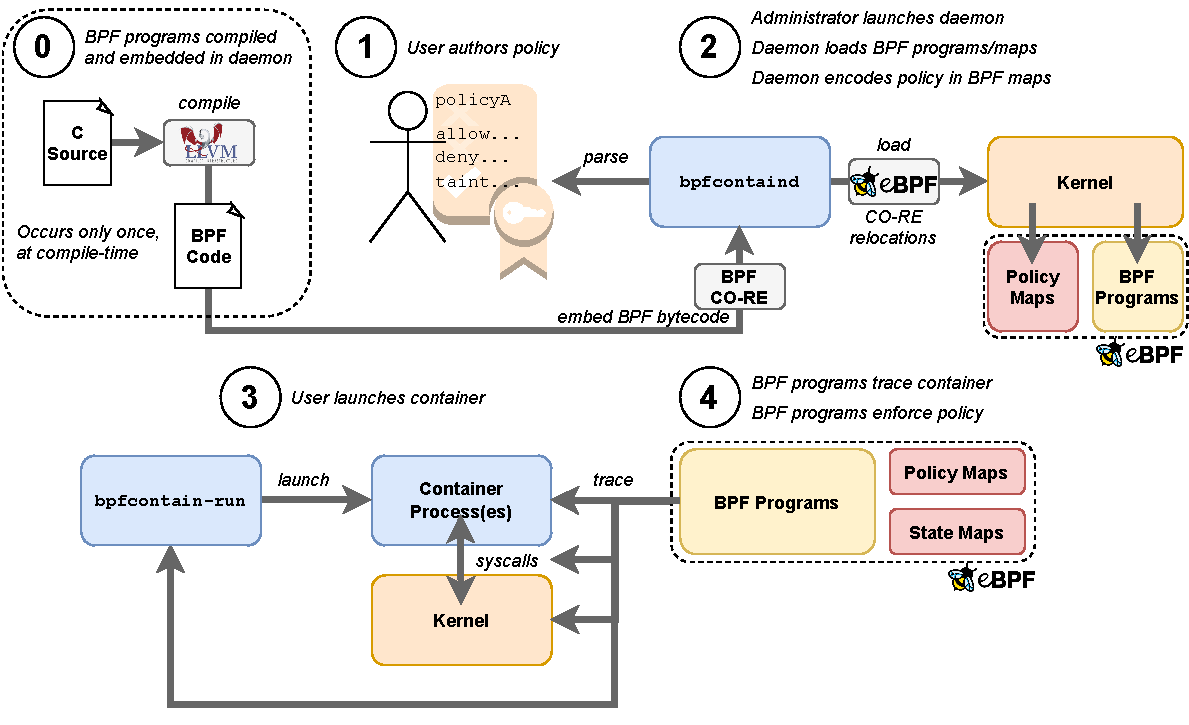
\includegraphics[width=1\linewidth]{figs/bpfcontain/overview.pdf}
  \caption[A high-level overview of how \bpfcontain{} confines applications]{
    A high-level overview of how \bpfcontain{} confines applications.  At compile-time,
    the object code for \bpfcontain{}'s \gls{bpf} programs is embedded directly into the
    resulting binary. To confine a container, the user first authors a high-level policy
    in their chosen data serialization language. The daemon parses this policy and loads
    it into the kernel by encoding it into \gls{ebpf} maps. The user then launches the
    container using the \texttt{bpfcontain-run} wrapper, at which point \bpfcontain{}
    begins tracing it and enforcing policy. Note the subtle differences between this
    figure and \Cref{fig:bpfbox-policy-overview} in \Cref{c:bpfbox}.
  }%
  \label{fig:bpfcontain-overview}
\end{figure}

The \bpfcontain{} daemon runs as a privileged process, parsing and loading user policy by
encoding it into a series of \gls{bpf} maps. The user then launches their container using
an unprivileged wrapper program, \texttt{bpfcontain-run}. The sole task of this wrapper
application is to invoke a stub function which does nothing more than pass the desired
policy ID as an argument. \bpfcontain{} traces this function call and uses it to confine
the container with the correct policy. Unlike \bpfbox{}, this technique enables the user
to associate any container with any policy, rather than a fixed one-to-one mapping.

At runtime, \bpfcontain{}'s \gls{bpf} programs trace the behaviour of processes running
under the container and confine it according to a mixture of default policy and policy
rules specified by the user. Like \bpfbox{}, enforcement is accomplished primarily through
\gls{bpf} programs attached to \gls{lsm} hooks in the kernel. The precise implementation
details of these programs vary significantly, and are covered in detail in
\Cref{s:bpfcontain-implementation}. \Cref{fig:bpfcontain-overview} illustrates
a high-level overview of the policy enforcement process described here.



\section{\bpfcontain{} Implementation}%
\label{s:bpfcontain-implementation}

This section presents the implementation details and architecture of \bpfcontain{}'s
policy enforcement mechanism. Specifically, we provide an initial overview of
\bpfcontain{}'s userspace and kernelspace components, then examine how \bpfcontain{}
enforces policy in the kernel using \gls{ebpf}. Whereas this section focuses specifically
on policy enforcement, \Cref{s:bpfcontain-policy} outlines and documents the details of
\bpfcontain{}'s policy language.

\subsection{Architectural Overview}%
\label{ss:bpfcontain-architecture}

Like \bpfbox{}, \bpfcontain{} is implemented as privileged daemon that runs in userspace
and loads \gls{ebpf} code into the kernel for policy enforcement. However, the precise
architecture and implementation details of this daemon are quite different. In particular,
the daemon is implemented in Rust and leverages the libbpf-rs crate\footnote{A crate is
a Rust package that can be added as a dependency to a project. For the purposes of this
thesis, we can consider the terms \enquote{crate} and \enquote{library} to be
equivalent.}~\cite{libbpf-rs} to load its \gls{ebpf} programs and maps into the kernel.
This results in a number of advantages, which we discuss in more detail in the following
section.

\bpfcontain{}'s kernelspace components are implemented in \gls{ebpf}. \gls{ebpf} programs
trace container lifecycle and enforce policy, while \gls{ebpf} maps store policy and pass
intermediary state between program invocations. This architecture is similar in spirit to
the design of \bpfbox{}, but with a few fundamental differences. Firstly, rather than
using the LLVM toolchain to compile programs at runtime, \bpfcontain{} pre-compiles and
embeds the \gls{bpf} object code into its binary object file. Using \gls{bpf}
\gls{core}~\cite{nakryiko2020_core}, these programs can then be dynamically loaded into
any supported kernel, regardless of the underlying configuration or architectural details.

\bpfcontain{} leverages several \gls{bpf} program and map types to implement container
tracing and confinement. While many of the major program types are shared with \bpfbox{},
there are a few distinct differences (c.f.~\Cref{ss:bpfbox-architecture} of
\Cref{c:bpfbox}). We enumerate these differences as follows. Map types are outlined in
\textbf{\green{green}} and program types are outlined in \textbf{\purple{purple}}.
\begin{itemize}
  \item \bpfcontain{} replaces many of \bpfbox{}'s \textbf{\green{Hash Maps}},
  particularly those used to track process state, with equivalent \textbf{\green{Local
  Storage Maps}}. Local storage is a new \gls{ebpf} map type supported in the latest
  kernels (Linux 5.11 and onwards). Local storage maps tether the underlying value to
  a kernel data structure, such as a task or inode, used as a key into the map. The result
  is a dynamically-allocated and garbage-collected per-structure storage blob.
  \bpfcontain{} leverages these for more memory-efficient storage of per-task and
  per-inode state.

  \item \bpfcontain{} replaces the use of scheduler \textbf{\purple{Tracepoints}} with
  equivalent \textbf{\purple{\gls{lsm} Probes}} that expose the same information. This
  reduces potential overhead from multiple \gls{bpf} program invocations on the same code
  path, most notably over \texttt{fork(2)} and \texttt{clone(2)} family system calls.

  \item \bpfcontain{} uses \textbf{\purple{Fentry and Fexit}} probes in place of
  \textbf{\purple{Kprobes}}. These use a more efficient trampoline technique for program
  entry and use \gls{btf} information exposed by the kernel for direct memory access,
  making them far more efficient than kprobes.
\end{itemize}

Aside from the aforementioned differences, \bpfcontain{} uses the same \gls{bpf} program
and map types as \bpfbox{}. However, the underlying implementation details of each
\gls{bpf} program will be quite different from \bpfbox{}, as \bpfcontain{} is dealing with
container semantics, new policy rules, and more nuanced policy defaults. We examine the
most important implementation details in the subsections that follow.



\subsection{Policy Deserialization and Loading}%
\label{ss:bpfcontain-serde}

\bpfcontain{} implements policy deserialization using Serde~\todo{CITE}, a data
serialization crate for Rust. Serde leverages Rust's powerful type system and procedural
macros to derive serialization and deserialization logic for vanilla Rust structs and
enums. Rust crates that consume Serde's \gls{api} can then use the automatically generated
logic for serialization and deserialization. This design enables a plug-and-play
relationship between a data schema, defined as a Rust data structure and any data
serialization language supported through the Rust crates ecosystem. \bpfcontain{} uses
Serde to automatically generate the accompanying deserialization logic for
a \texttt{Policy} struct and several \texttt{Rule} structs, one for each supported rule
type. \Cref{lst:bpfcontain-serde} depicts a simplified example of how this works.

\begin{lstlisting}[language=Rust, gobble=2, caption={[A simplified example of \bpfcontain{}'s policy deserialization logic]
  A simplified example of \bpfcontain{}'s policy deserialization logic. Policy rules are
  specified declaratively using Rust structs and the corresponding deserialization logic
  is automatically generated by the Serde crate, using a simple decorator macro.
},
label={lst:bpfcontain-serde}]
  use serde::Deserialize;

  /// The policy data structure
  #[derive(Deserialize)]
  pub struct Policy {
    name: String,
    /* Other policy metadata would go here... */
    allow: Vec<Rule>,
    deny: Vec<Rule>,
    taint: Vec<Rule>,
  }

  /// An enum encompassing all rule types
  #[derive(Deserialize)]
  pub enum Rule {
    FileRule(FileRule),
    /* Other rule types would go here... */
  }

  /// A "file access" rule
  #[derive(Deserialize)]
  pub struct FileRule {
    pathname: String,
    access: String,
  }

  /* Other rule types would go here... */
\end{lstlisting}

To enable the daemon to encode policy as an \gls{ebpf} map, each rule type implements the
\texttt{LoadableRule} trait. The daemon uses this logic to convert a policy rule into
a canonical format that can be represented in the kernel and thus used to enforce security
policy. Implementing this trait is as simple as writing a \texttt{load()} function that
makes a series of map updates to load the rule into the kernel; we leverage
libbpf-rs~\cite{libbpf-rs} for this purpose. When loading a policy into the kernel, the
daemon simply invokes this \texttt{load()} function for each policy rule.

Implementing policy deserialization and loading logic in this way has a number of
advantages. Since the policy schema is simply encoded declaratively in vanilla Rust, it is
easy for a developer (even a new contributor to \bpfcontain{}) to implement a new rule
type and add it to \bpfcontain{}. Adding a new rule type is as simple as defining a new
Rust data type to represent the rule and implementing the \texttt{LoadableRule} trait,
enabling the daemon to encode the rule as an \gls{ebpf} map. Due to Serde's modular
design, supporting a new serialization language for \bpfcontain{} policies is trivial; we
simply pull in the corresponding consuming crate as a dependency. Currently, \bpfcontain{}
supports YAML, JSON, and TOML as policy language encodings, but this can easily be
extended in future versions.

\subsection{Policy Enforcement}%
\label{ss:bpfcontain-enforcement}

Policy enforcement under \bpfcontain{} can be thought of as a combination of
\textit{explicit policy} (the rules defined in the policy file) and a nuanced
\textit{default policy} (the set of sensible defaults that \bpfcontain{} enforces to
define a boundary around the container). \todo{Explain in more details}

\todo{Have a list of steps here, similar to that of \bpfbox{}.}
\begin{enumerate}
  \item
\end{enumerate}

\subsection{Default Policy}%
\label{ss:bpfcontain-default}

\subsection{Managing Container State}%
\label{ss:bpfcontain-state}

\subsection{Collecting and Logging Audit Data}%
\label{ss:bpfcontain-audit}




\section{\bpfcontain{} Policy Language}%
\label{s:bpfcontain-policy}

\todo{This section will present and document the policy language of \bpfcontain{}, taken from our paper.}

\subsection{File, Filesystem, and Device Rules}

\subsection{Network Rules}

\subsection{\glsentryshort{ipc} Rules}

\subsection{Capability Rules}

\subsection{Allow, Deny, and Taint Policy}




\section{Improvements Over \bpfbox{}}%
\label{s:bpfcontain-improvements}

\subsection{Minimizing Runtime Dependencies}%
\label{ss:bpfcontain-minimizing}

\begin{inprogress}
\bpfcontain{} solves \bpfbox{}'s dependency and runtime overhead issues by leveraging Rust
and libbpf \gls{core}~\cite{nakryiko2020_core} rather than Python and bcc.  Unlike bcc,
libbpf \gls{core} enables \gls{bpf} programs to be compiled once and run anywhere, thanks
to \gls{btf} information provided by the kernel and load-time symbol relocation. Program
bytecode can then be embedded directly into the compiled object file, meaning the single
pre-compiled \bpfcontain{} binary can be deployed on any target kernel that meets
a minimal set of requirements. As a side effect, \bpfcontain{} requires neither a full
LLVM toolchain nor kernel headers to be available in the target deployment, significantly
reducing the dependency overhead.

Moreover, implementing the \bpfcontain{} daemon in Rust allows \bpfcontain{} to take
advantage of a myriad of benefits offered by the Rust language. In particular, Rust
enables \bpfcontain{}'s userspace components to be safe, secure, and fast. Thread- and
memory-safety guarantees provided by Rust ownership model eliminate many common security
bugs including memory corruption vulnerabilities and race conditions between threads.
These safety guarantees provide critical security advantages, particularly given the fact
that the \bpfcontain{} daemon is a long-running, privileged process\,---\,a ripe target
for attacker exploitation. Thanks to an emphasis on speed and zero-cost abstractions, Rust
can provide these benefits at virtually zero overhead, in line with traditional systems
programming languages like C and significantly better than languages with a bulky runtime
such as Python.
\end{inprogress}

\subsection{Simplified Policy Language}%
\label{ss:bpfcontain-simplified}

\begin{inprogress}
To rectify these issues in the policy language design, \bpfcontain{} eschews the original
policy language and instead reaches for a more modular approach.  Rather than defining an
entire new policy language, \bpfcontain{} instead defines a policy language
\textit{schema}. This schema can then be encoded in any number of available data
serialization formats, including YAML~\todo{CITE}, JSON~\todo{CITE}, TOML~\todo{CITE} and
others. The end result is that the user is able to choose whichever policy encoding they
are most comfortable with, using serialization languages that are both commonly available
and that have stood the test of time across a variety of production use cases. Another
implicit advantage of this approach is that it enables the future integration of
\bpfcontain{} policy into existing container specification schemas, such as the \gls{oci}
specification, which is encoded in JSON\@.
\end{inprogress}

\subsection{Container-Specific Extensions}%
\label{ss:bpfcontain-extending}

\todo{This section will discuss how \bpfcontain{} extends \bpfbox{} to model containers.
Specifically, the idea is to enforce policy at the granularity of an entire container
rather than an individual process. This lets us get away with all sorts of default
policy\,---\,all operations within the confines of the container that do not affect the
rest of the system are permitted. Operations that impact the rest of the system, such as
those that modify kernel code, system parameters, or similar are denied. Everything else
can be specified as a rule. This basically allows us to get away with almost no policy
language whatsoever. A nice way to put it: \enquote{The policy language is used to define
the exceptions rather than the rules}.}

\begin{inprogress}
\bpfcontain{} rectifies this gap by incorporating container semantics into the design of
both its policy language and enforcement engine. This includes properties such as
namespace and container membership, defining an implicit boundary around the container and
related resources, similar in spirit to FreeBSD Jails~\cite{kamp2000_jails}. In this way,
\bpfcontain{} policies can grant access to objects that exist within the container and
revoke access to objects that exist outside the container. Policies then focus on defining
exceptions to this boundary, exposing fine-grained interfaces into the container and
locking down the rest by default.
\end{inprogress}




\section{Summary}%
\label{s:bpfcontain-summary}

\todo{Summary here.}



\todo{Add the three design goals here by fulfillment?}
\begingroup
\begin{longtable}[c]{llll}
\caption[Comparing \bpfbox{} and \bpfcontain{}]{
    Comparing \bpfbox{} and \bpfcontain{} by their properties and how well each satisfies
    the design goals outlined in \Cref{s:cp-design}.
}%
\label{tab:bpfcontain-comparison}\\
  \toprule
                 & Userspace        & Kernelspace & Dependencies \\
  \midrule
  \bpfbox{}      & Python + bcc     & bcc & High \\
  \bpfcontain{}  & Rust + libbpf-rs & \glsentryshort{bpf} \glsentryshort{core} & Minimal \\
  \bottomrule
\end{longtable}
\endgroup
